\chapter{LHC and the CMS experiment}
\chaptermark{The LHC and the CMS experiment}  
\thispagestyle{plain}  % First page has default style
\pagestyle{chapterpages}
\label{Section:Chapter3}

The physics analyses presented in this thesis are performed using data generated by the LHC and collected by the \ac{CMS} experiment. This chapter begins by exploring how the LHC accelerates and collides protons up to centre-of-mass energies ($\sqrt{s}$) of $13.6\TeV$, creating the extreme but necessary conditions needed for rigorous tests of the SM at the electroweak scale. The discussion then shifts to the CMS detector, a multipurpose apparatus composed of several layers of specialised subdetectors. These intricate systems work in concert to enable the precise reconstruction of particles emerging from proton-proton collisions at the heart of the detector.

\section{The LHC}

The LHC~\cite{LHC_1}, situated at the European Organization for Nuclear Research (CERN) near Geneva, Switzerland, is a testament to human scientific achievement. Ingeniously, the LHC was placed within the tunnel previously occupied by the Large Electron Positron (LEP) collider. Engineered to facilitate proton-proton (pp) collisions, the machine was designed to generate such collisions with centre-of-mass energy up to $14\TeV$ and an unprecedented luminosity of $10^{34}\unit{cm}^{-2}\unit{s}^{-1}$. As mentioned earlier, the LHC is currently running just below its maximum energy capabilities, with each beam carrying $6.8\TeV$ of energy. Spanning a circumference of $27\unit{km}$, the LHC mirrors the basic layout of its predecessor, LEP, as illustrated in Fig~\ref{Figure:Chapter3_LHC_BasicLayout}. 

\begin{figure}[h]
\centering
\includegraphics[width= 0.7\textwidth]{Figures/Chapter3/LHC_BasicLayout.jpg}
\caption{Basic schematic layout of the LHC consisting of 8 arc sections along with the two circulating beams and the ATLAS, ALICE, CMS, and LHCb experiments~\cite{LHC_BasicLayout}.}
\label{Figure:Chapter3_LHC_BasicLayout}
\end{figure}

The experimental landscape is strategically arranged with two general-purpose experiments, ATLAS~\cite{LHC_ATLAS} and CMS~\cite{LHC_CMS}, positioned at diametrically opposite sections, at Points 1 and 5 respectively. The ALICE experiment~\cite{LHC_ALICE} occupies Point 2, while LHCb~\cite{LHC_LCHb} is situated at Point 8. At these critical locations, the circulating beams are precisely focused and brought into collision.

Particles are not accelerated to an energy of $6.8~\TeV$ per beam simply by circulating in the LHC tunnel. Instead, the LHC is the final stage of a sophisticated accelerator chain~\cite{LHC_InjectorComplex} at CERN, in which a series of machines successively boost the energy of the particles, as shown in Fig.~\ref{Figure:Chapter3_LHC_Complex}. The first step in this accelerator complex is the Linear Accelerator 4 (LINAC4)~\cite{LINAC4}, which produces a beam of negative hydrogen ions ($\text{H}^-$), each consisting of a proton and two electrons. LINAC4 accelerates these ions to an energy of $160\MeV$ before injecting them into the Proton Synchrotron Booster (PSB). During injection, the electrons are stripped off, leaving behind bare protons. The PSB then accelerates the protons to a kinetic energy of $2.0\GeV$. Next, the beam is transferred to the Proton Synchrotron (PS), which increases its energy to $26\GeV$. From there, the particles are sent to the largest machine in the injector complex, the Super Proton Synchrotron (SPS), which boosts their energy to $450\GeV$. Throughout the injector chain, the protons are grouped into bunches, which are subsequently injected into the two concentric beam pipes of the LHC as two counter-rotating beams. The injection continues until each beam consists of 2808 bunches, separated by $25\unit{ns}$.

\begin{figure}[h]
\centering
\includegraphics[width= 1.0\textwidth]{Figures/Chapter3/LHC_AcceleratorComplex.png}
\caption{Schematic diagram of the CERN accelerator complex~\cite{LHC_InjectorComplex}.}
\label{Figure:Chapter3_LHC_Complex}
\end{figure}

A network of 1232 superconducting (niobium-titanium) dipole magnets bend the beams along the circular LHC ring. These magnets operate at ultra-low temperatures of $1.9\unit{K}$, achieved using superfluid helium, and can produce magnetic fields up to $8.4\unit{T}$. Beam acceleration is facilitated by sixteen $400\unit{MHz}$ radiofrequency (RF) cavities, providing a \~14-fold energy increase compared to the injection energy. The circular trajectory of the accelerating beams is maintained by dynamically adjusting the magnetic field strength of the dipole magnets, while 392 quadrupoles are utilised to focus the beams. Just before the collision at each of the four principal points, four inner triplet quadrupole magnets are used to reduce the transverse size of the beams. This effectively squeezes them, aiming to maximise the collision rate~\cite{LHC_Run3}, as illustrated in Fig.~\ref{Figure:Chapter3_LHC_BeamSqueeze}. The specifications mentioned above reflect the state of the accelerator complex following the upgrades carried out during the latest scheduled long shutdown, which was completed in 2021.

\begin{figure}[h]
\centering
\includegraphics[width= 0.7\textwidth]{Figures/Chapter3/LHC_BeamSqueeze.pdf}
\caption{Illustration of beam squeezing prior to colliding in the heart of detectors at the LHC.}
\label{Figure:Chapter3_LHC_BeamSqueeze}
\end{figure}

\subsection{Cross section and Luminosity}

Cross section and luminosity are essential in understanding and measuring what happens in collider collisions. Together, these determine how often specific physical processes occur in the detector. The cross-section ($\sigma$) describes the probability of a particular process occurring during a collision. Many different processes can occur as the beams cross in the heart of the LHC detectors. The cross-section of each of these processes depends on the type and the energy of the colliding particles, $\sigma(\sqrt{s})$. The cross-section is combined with the instantaneous luminosity ($\mathscr{L}$) to calculate how often a particular process occurs at a collider. Instantaneous luminosity is a measure of how tightly particles are packed into a given space, and it is a function of the beam parameters~\cite{LHC_HL},

\begin{equation}
\begin{aligned}
    \mathscr{L} &= \gamma \frac{n_b N^2 f_{\text{rev}}}{4\pi \beta^* \epsilon_n} R \\
    R &= 1 / \sqrt{1 + \left( \frac{\theta_c \sigma_z}{2\sigma} \right) }
\end{aligned}
\end{equation}

where $\gamma$ is the proton beam energy expressed in rest mass units, $n_b$ is the number of bunches per beam, $N$ is the number of particles per bunch, $f_{rev}$ is the revolution frequency ($11.2\unit{kHz}$), $\beta^*$ is the beam beta function at the collision point and $\epsilon_n$ is the normalised transverse beam emittance. The term R is a geometrical reduction factor for luminosity. This is expressed as a function of the crossing angle of the beams at the collision point ($\theta_c$) and the transverse (longitudinal) spread of the particle bunch, $\sigma_z(\sigma)$. 

The cross-section, together with the instantaneous luminosity, determines the rate (R) at which a given process occurs in the detector,

\begin{equation}
    R = \sigma(\sqrt{s}) \cdot \mathscr{L} 
\end{equation}

The beam parameters are constant over time; hence, the luminosity varies. A more appropriate quantity is the integrated luminosity ($\mathscr{L}_{int}$), which considers the total data collected over a given period,

\begin{equation}
    \mathscr{L}_{int} = \int \mathscr{L}(t) dt
\end{equation}

In a given period, the total number of events (N) for a particular process with cross-section $\sigma$ can be expressed as:

\begin{equation}
    \mathscr{N} = \sigma \cdot \mathscr{L}_{int}
\end{equation}

A summary of the total integrated luminosity delivered to the CMS experiment since 2015 is provided in Fig.~\ref{Figure:Chapter3_CMS_IntegratedLumi}.

\begin{figure}[h]
\centering
\includegraphics[width= 0.7\textwidth]{Figures/Chapter3/CMS_IntegratedLumi.pdf}
\caption{Total integrated luminosity delivered to the CMS experiment between 2015 and 2024. Data collected from all periods except 2015 and 2024 are used in this thesis. The figure is taken from Ref.~\cite{CMS_IntegratedLumi}.}
\label{Figure:Chapter3_CMS_IntegratedLumi}
\end{figure}

\subsection{Pileup}

The CMS experiment set out to investigate the rarest interactions of proton collisions. In the effort of maximising the chances of observing such rare events, the LHC collides large bunches of protons rather than single protons, as discussed earlier. This approach increases the instantaneous luminosity, which is favourable because it directly enhances the probability of rare processes occurring within a given time. However, this also introduces challenges: when bunches collide, multiple protons interact simultaneously. In other words, CMS records particles from the interaction of interest and particles originating from multiple additional interactions, called pileup interactions. Increasing the instantaneous luminosity leads to the enhancement of pileup. The removal of these unwanted overlap collisions requires increasingly more sophisticated techniques. Figure~\ref{Figure:Chapter3_CMS_Pileup} illustrates the pileup conditions encountered by the CMS experiment between 2015 and 2024.

\begin{figure}[h]
\centering
\includegraphics[width= 0.7\textwidth]{Figures/Chapter3/CMS_Pileup.pdf}
\caption{Distribution of average number of interactions per crossing for pp collisions between 2015 to 2024 using data from the CMS experiment, taken from Ref.~\cite{CMS_IntegratedLumi}.}
\label{Figure:Chapter3_CMS_Pileup}
\end{figure}

\section{The CMS Detector}
\label{Section:Chapter3_CMS_Detector_Introduction}
As previously discussed, CMS is one of the two general-purpose detectors at the LHC, built to explore a wide range of high-energy physics phenomena. The design of the CMS detector was shaped by the ambitious goals of the LHC physics programme, which demanded precise and efficient measurements under challenging experimental conditions. To accomplish these objectives, several key performance requirements were identified:

\begin{itemize}
    \item Identification and precise momentum reconstruction of muons over a broad range of momenta and angles. A dimuon mass resolution of approximately 1\% at 100$\GeV$ is required, along with the ability to determine the charge of muons with momenta below 1$\TeV$ unambiguously.

    \item Good momentum resolution and reconstruction efficiency for charged particles in the inner tracking system. Efficient identification of $\tau$ leptons and b-jets necessitates fine granularity tracking, which is required to locate signatures consistent with secondary interaction vertices.

    \item Electromagnetic energy measurements with excellent resolution for photons and electrons. Diphoton and dimuon mass resolutions of approximately 1\% at 100$\GeV$ are required over a wide geometrical coverage.

    \item Effective $\pi^0$ rejection to distinguish isolated photons from those originating in neutral pion decays. Additionally, efficient isolation of photons and leptons is required, particularly in high-luminosity environments with significant detector occupancy.

    \item Good dijet mass and \ac{MET} resolution are required, necessitating fine laterally segmented hadronic calorimeters providing a near-complete hermetic coverage.
\end{itemize}

CMS employs a compact, layered detector system arranged cylindrically around the interaction point to fulfil these performance requirements, providing a near-complete solid-angle coverage. The entire detector is $21.6\unit{m}$ long and has a diameter of $14.6\unit{m}$ while weighing $12500\unit{t}$. This makes CMS one of the most massive yet \textbf{compact} detectors ever engineered for a particle physics experiment. Closest to the beam pipe lies the silicon tracker, which precisely tracks charged particles. It is surrounded by the Electromagnetic Calorimeter (ECAL), optimised for measuring the energy of electrons and photons with high precision. The Hadronic Calorimeter (HCAL) follows and is responsible for absorbing and measuring the energy of hadrons. These three subsystems are enclosed within a powerful $13\unit{m}$ long, $6\unit{m}$ inner-diameter, $3.8\unit{T}$ superconducting \textbf{solenoid}. Embedded within the iron return yoke of the solenoid is the \textbf{muon} detection system. A schematic of the full CMS detector is shown in Fig.~\ref{Figure:Chapter3_CMS_schematic}, providing an overview of its cylindrical geometry and layered structure around the LHC interaction point. The following sections will discuss each of the major detector subsystems introduced here in more detail. A complementary longitudinal slice through the detector is shown in Fig.~\ref{Figure:Chapter3_CMS_slice}, serving as a visual reference for the detailed subsystem descriptions that follow.

\begin{figure}[h]
\centering
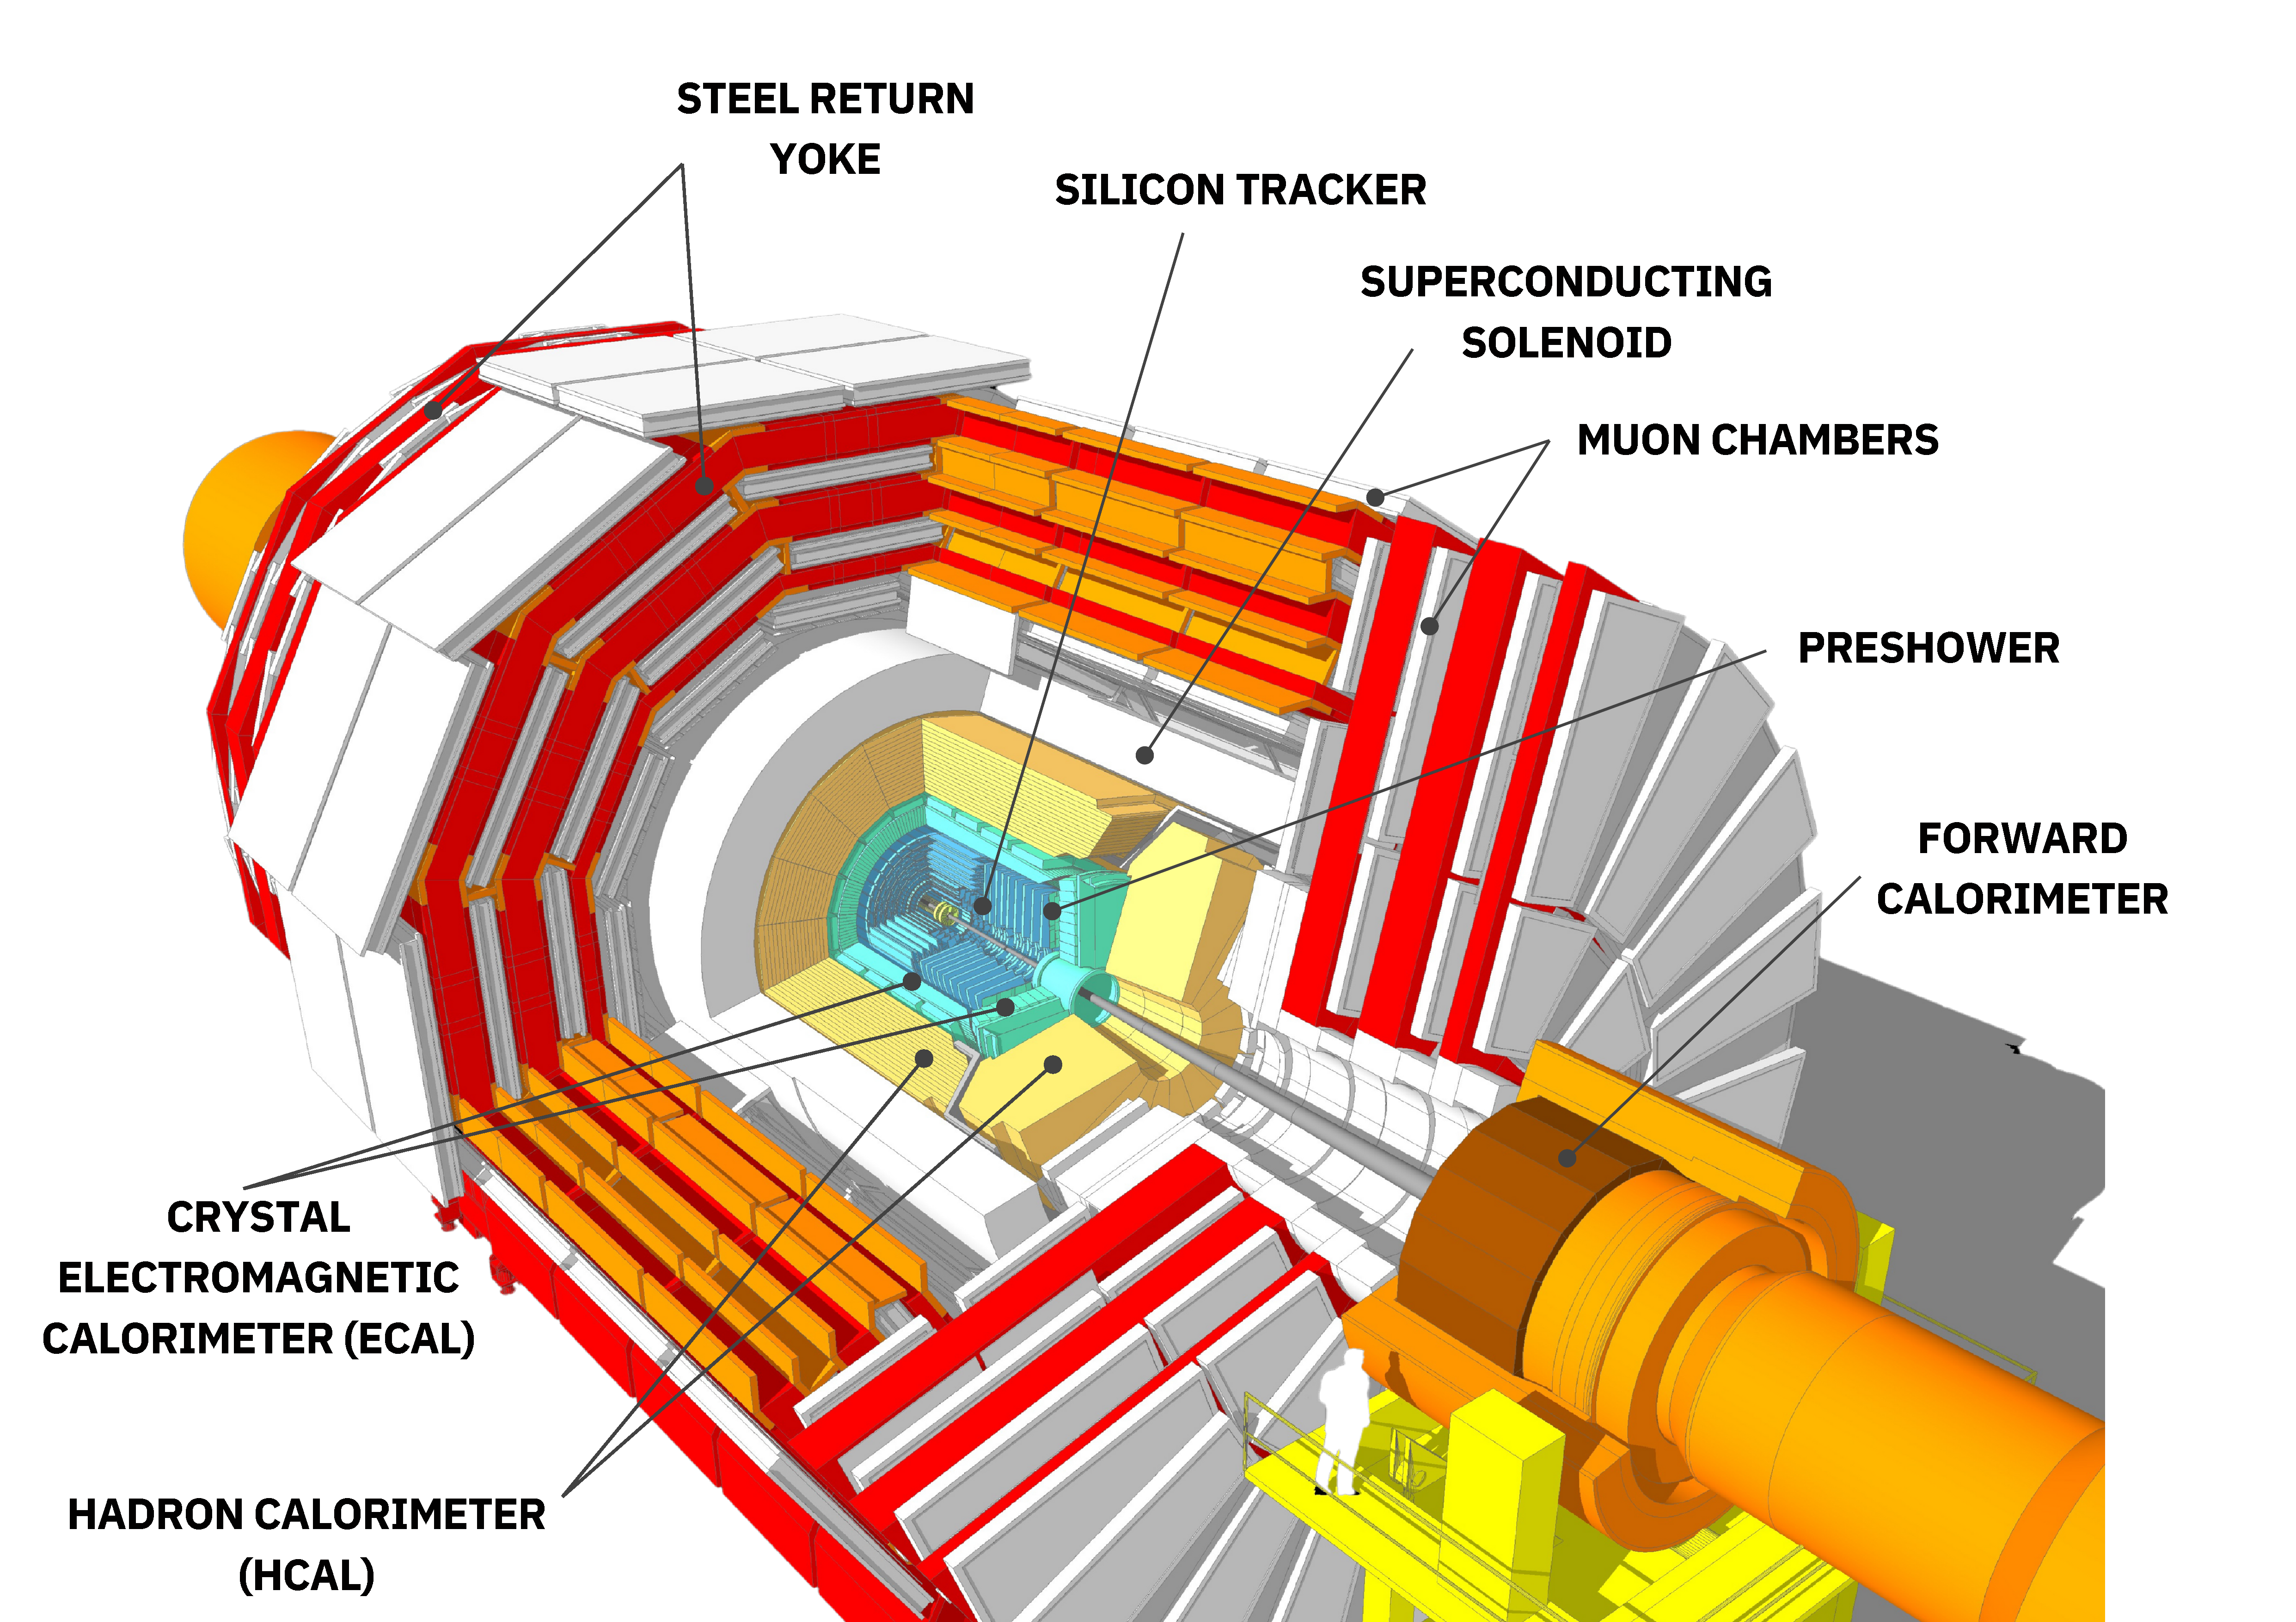
\includegraphics[width= 1\textwidth]{Figures/Chapter3/CMS_Detector.png}
\caption{Schematic drawing of the CMS detector taken from Ref.~\cite{CMS_Detector_Run3}.}
\label{Figure:Chapter3_CMS_schematic}
\end{figure}

\begin{figure}[h]
\centering
\includegraphics[width= 1\textwidth]{Figures/Chapter3/CMS_Detector_Slice.pdf}
\caption{A transverse slice of the CMS detector displaying the individual subsystems and their response to different types of particles. The figure is taken and adjusted from Ref.~\cite{CMS_Detector_Slice}.}
\label{Figure:Chapter3_CMS_slice}
\end{figure}

\subsection{Co-ordinate system}
The CMS detector adopts a right-handed Cartesian coordinate system centred at the nominal collision point inside the detector. The x-axis points towards the centre of the LHC ring, and the y-axis points vertically upwards, while the z-axis points along the beam direction towards the Jura mountains, as illustrated in Fig~.\ref{Figure:Chapter3_CMS_CoordinateSystem}.

\begin{figure}[h]
\centering
\includegraphics[width= 1\textwidth]{Figures/Chapter3/CMS_CoordinateSystem.png}
\caption{The CMS detector coordinate system.}
\label{Figure:Chapter3_CMS_CoordinateSystem}
\end{figure}

In addition to the Cartesian coordinate system (x,y,z), it is often convenient to describe particle kinematics using cylindrical coordinates. In this system, the azimuthal angle ($\phi$) is measured from the x-axis in the (x-y) plane, spanning the range $|\phi| < \pi$. The polar angle is measured from the z-axis in the (z-y) plane, while r is the radial distance in the (x-y) plane. Rather than using the polar angle ($\theta$) directly, it is common in collider physics to introduce pseudorapidity ($\eta$), which is defined in terms of $\theta$ as:

\begin{equation}
    \eta = - \ln[\tan(\theta/2)]
\end{equation}

A key property of pseudorapidity is that the difference in $\eta$ between two particles is invariant under Lorentz boosts along the z-axis. This property is extremely useful in collider experiments where the parton-parton centre-of-mass frame can often be significantly boosted along the beam direction due to the variable momentum fractions carried by the incoming partons. Additionally, pseudorapidity provides a nearly linear mapping of detector geometry, aligning naturally with the physical segmentation of the detector into barrel and endcap regions.

\begin{itemize} 
\item Barrel region: The central cylindrical region of the detector, located closest to the primary interaction point and optimised for particles emitted at large angles to the beamline ($\ie$ low $|\eta|$). 
\item Endcap regions: Located at either end of the barrel along the z-axis, designed to detect particles emitted at small angles with respect to the beamline ($\ie$ high $|\eta|$). 
\end{itemize}

The distance metric in these coordinates ($\eta$-$\phi$) can be defined as:

\begin{equation}
    \Delta R = \sqrt{(\Delta\eta)^2 + (\Delta \phi)^2}
\end{equation}

At the LHC, the initial momentum component of the system perpendicular to the beam axis is nearly zero because of the head-on nature of the beam. This kinematic quantity is referred to as the transverse momentum ($p_T$) and is defined as:

\begin{equation}
    p_T = \sqrt{p_x^2 + p_y^2}
\end{equation}

Transverse momentum is a central observable in collider physics, as it provides a direct probe of hard interaction processes characterized by large momentum transfers. A complementary quantity to the transverse momentum is the missing transverse momentum ($E_T^{\text{miss}}$), which is defined as the negative vector sum of the transverse momenta of all reconstructed particles in an event. This is a critical quantity serving as an estimator of the transverse momentum carried by non-interacting or undetected particles.

\subsection{Magnet System}

As its name implies, the CMS is defined by its central feature—the Compact Muon Solenoid. This critical component generates a powerful magnetic field that bends the trajectories of charged particles as they traverse the detector, enabling precise measurements of their momenta and electric charges. This capability is crucial for achieving the 1\% dimuon mass resolution at 100$\GeV$ and for unambiguous charge determination of muons with momenta below 1$\TeV$, as outlined in the performance requirements.

The solenoid spans $13\unit{m}$ in length and $6\unit{m}$ in diameter, able to produce a magnetic field of up to $4\unit{T}$ but, currently operated at $3.8\unit{T}$ for enhanced long-term stability. The strong field ensures that low-momentum charged particles are sufficiently curved, confining them within the inner tracking system and aiding in precise momentum resolution. This not only improves tracking quality but also helps mitigate calorimeter noise by preventing soft particles from reaching the calorimeters.

To contain the magnetic flux, an iron return yoke surrounds the solenoid. This massive structure, weighing approximately $10000\unit{t}$, not only completes the magnetic circuit but also houses the muon detection system, embedded within its segmented layers. This configuration enables double bending of muon trajectories—first within the silicon tracker and again within the muon stations, enhancing the overall muon momentum resolution.

\subsection{Inner tracking system}

The interaction point in the CMS experiment is surrounded by the innermost sub-detector, the silicon tracker, measuring at 5.8$\unit{m}$ long with a diameter of 2.5$\unit{m}$~\cite{LHC_CMS,CMS_Detector_Run3}. The tracker is essential for precisely measuring the trajectories of charged particles and the determination of primary and secondary interaction vertices. At design luminosity, $\mathcal{O}(10^3)$ particles traverse its active volume in each bunch crossing (25$\unit{ns}$); hence, it is required to have a high granularity and fast response to meet the LHC and the CMS physics requirements. The tracker is exposed to an extremely harsh radiation environment near the interaction, requiring its components to be radiation-hard to maintain performance despite their prolonged exposure to ionising radiation. The CMS experiment adopted silicon-based trackers to meet these demands. Although silicon sensors are thin, they require dedicated readout electronics and active cooling, which contribute significantly to the non-active material within the tracker volume. Minimising this non-active material is essential, as it increases multiple scattering and energy loss, degrading track and momentum resolution and ultimately affecting calorimeter performance. As shown in Fig.~\ref{Figure:Chapter3_Tracker_MaterialBudget}, the tracker material budget is kept particularly low in the central (low-$\eta$) region of the pixel sub-detector.

\begin{figure}[h]
    \centering
    % First row
    \begin{subfigure}[b]{0.49\textwidth}
        \centering
        \includegraphics[width=\textwidth]{Figures/Chapter3/Material_Budget1.pdf}
        \caption{}
    \end{subfigure}
    \begin{subfigure}[b]{0.49\textwidth}
        \centering
        \includegraphics[width=\textwidth]{Figures/Chapter3/Material_Budget2.pdf}
        \caption{}
    \end{subfigure}
\caption{Simulation of the CMS pixel detector material budget as a function of $\eta$ in units of ($\textbf{a}$) radiation length and ($\textbf{b}$) hadronic interaction length for different detector components~\cite{TrackerMaterialBudget_Pixel}.}
\label{Figure:Chapter3_Tracker_MaterialBudget}
\end{figure}


\subsubsection{Pixel Detector}
The innermost component of the CMS tracking system is the silicon pixel detector. The original detector~\cite{LHC_CMS}, installed in 2008, was designed to operate for up to ten years under the LHC’s nominal instantaneous luminosity of $1 \times 10^{34}~\unit{cm}^{-2}\unit{s}^{-1}$, with the capacity to handle up to 25 inelastic proton-proton interactions per bunch crossing (PU). However, even during Run~1, the LHC exceeded its design luminosity, exposing the detector to higher radiation levels and increasing readout inefficiencies.

To maintain high tracking efficiency under luminosity conditions up to $2 \times 10^{34}~\unit{cm}^{-2}\unit{s}^{-1}$ and pileup levels of 50 or more, the CMS pixel detector underwent a significant upgrade in 2017, known as the Phase-1 upgrade \cite{CMS_Detector_Run3, CMS_Tracker_Phase1_Upgrade}. The upgraded pixel detector features four barrel layers (BPIX) located at radii of 29, 68, 109, and 160~$\unit{mm}$ (L1–L4), along with three endcap disks (FPIX) situated at 291, 396, and 516~$\unit{mm}$ from the detector centre. In total, 1184 silicon sensor modules are deployed in the barrel region and 672 in the forward region. Each module consists of a silicon sensor segmented into $160 \times 416$ pixels, with a pixel pitch of $100 \times 150~\unit{\mu m}^2$, yielding approximately 124 million readout channels.

As illustrated in Fig.~\ref{Figure:Chapter3_Pixel_Upgrade}, the Phase-1 upgrade also brought the innermost layer (L1) closer to the interaction point, made possible by reducing the beam pipe radius from 30 to 23~$\unit{mm}$ in 2014. This revision enhances the detector's acceptance and enables four-hit coverage (as opposed to three in the original configuration) for charged particle tracks within $|\eta| < 3.0$.

\begin{figure}[h]
\centering
\includegraphics[width= 1\textwidth]{Figures/Chapter3/CMS_Pixel_Upgrade.pdf}
\caption{Longitudinal view of CMS pixel detector comparing its structure before (lower part) and after (upper part) the Phase-1 Upgrade~\cite{LHC_Run3}.}
\label{Figure:Chapter3_Pixel_Upgrade}
\end{figure}

The upgraded system delivers a transverse ($r$–$\phi$) spatial resolution of approximately $11(12)~\unit{\mu m}$ and a longitudinal ($z$) resolution of around $24(21)~\unit{\mu m}$ in the barrel (forward region). Its increased granularity facilitates the three-dimensional reconstruction of charged particle trajectories, which is crucial for precise primary and secondary vertex determination. These capabilities also significantly enhance pileup mitigation and jet flavour tagging, both of which are central to physics analyses at high-luminosity conditions.

\subsubsection{Silicon Strip Tracker}

Surrounding the pixel detector is the silicon strip tracker (SST), illustrated in Fig.~\ref{Figure:Chapter3_Tracker_Geometry}. Silicon strips are chosen over pixels because of the reduced particle occupancy in the outer tracker, softening the granularity requirements. The strip tracker covers an active area of around $198\unit{m}^2$ with 9.3 million silicon micro-strips distributed over 15148 modules. It is composed of four subsystems. The Tracker Inner Barrel (TIB) is composed of four barrel layers, supplemented by three Tracker Inner Disks (TID) at each end, extending the coverage to $r < 550\unit{mm}$ and $|z| < 1180\unit{mm}$. The Tracker Outer Barrel (TOB) further extends the radius coverage ($r>550\unit{mm}$) and consists of six barrel layers. In the forward regions, the Tracker EndCaps (TEC) cover the region $1240 < |z| < 2820\unit{mm}$. Each TEC is composed of nine disks, each containing up to seven concentric rings of silicon strip modules.

\begin{figure}[h]
\centering
\includegraphics[width= 1\textwidth]{Figures/Chapter3/Phase1_Tracker.pdf}
\caption{Schematic view of one-quarter of the CMS inner tracking system in the (r-z) plane. The pixel detector is shown in green close to the beamline. Single-sided and double-sided stip modules are depicted as red and blue segments, respectively~\cite{CMS_Detector_Run3}. }
\label{Figure:Chapter3_Tracker_Geometry}
\end{figure}

In the barrel sections, the modules are configured to measure radial $r-\phi$ coordinates, while those in the TECs and TIDs are primarily oriented to measure $\phi-z$ coordinates. To accommodate the varying radiation environment and particle flux across the tracker volume, both the strip pitch and sensor thickness are adapted accordingly to maintain high spatial resolution and radiation tolerance. In the innermost two layers of the TIB and the TOB, as well as the modules in the first two rings of the TID, and rings 1, 2, and 5 of the TEC, a second strip detector module is installed. This module is mounted back-to-back with a ``stereo'' angle of $100\unit{mrad}$. The combination of hits from these two modules can provide additional measurements of the $z$ coordinate in the barrel and $r$ in the disks.

\subsection{Electromagnetic calorimeter}

As outlined by the LHC physics requirements in Section~\ref{Section:Chapter3_CMS_Detector_Introduction}, precise reconstruction of electromagnetic particles and robust suppression of background processes ($\pi^0 \to \gamma \gamma$) are essential for a detector like CMS.  The CMS Electromagnetic Calorimeter (ECAL)~\cite{LHC_CMS,CMS_Detector_Run3,CMS_ECAL_Performance_Run2} is designed to meet these demands, providing high-resolution energy measurements for electrons and photons. The ECAL is a hermetic homogeneous calorimeter consisting of 61,200 lead tungstate (PbWO$_4$) crystals mounted in the central barrel part and 7,324 crystals sorted in each of the two endcaps. The selection of radiation-hard PbWO$_4$ crystals for use at the LHC is driven by their characteristics. Specifically, their high density ($8.28\unit{gcm}^{-3}$), short radiation length ($0.89\unit{cm}$), and small Moli\`ere radius ($2.2\unit{cm}$) allow for a compact and finely granular calorimeter. In addition, these crystals exhibit a fast response time with approximately 80\% of the total scintillation light emitted in $25\unit{ns}$. This matches the LHC bunch crossing time, enabling the collection of most energy before the next proton bunch crossing.

A crucial component of the CMS ECAL is the photodetectors, which read out the scintillation light produced by electromagnetic showers in the crystals. The crystals’ relatively low light yield is one of their disadvantages, requiring photodetectors that can provide internal amplification while being insensitive to particles traversing them. These photodetectors must also be fast, radiation tolerant, and capable of operating within the $3.8-4\unit{T}$ longitudinal magnetic field. To meet these requirements, avalanche photodiodes (APDs) are used in the barrel region, offering a high internal gain. Conversely, vacuum phototriodes (VPTs) are employed in the endcap regions, which, while offering lower quantum efficiency and internal gain, exhibit a higher radiation tolerance.

As shown in Figures~\ref{Figure:Chapter3_CMS_schematic}-\ref{Figure:Chapter3_CMS_slice}, the ECAL is placed outside of the inner tracker. It is divided into a barrel region (EB), an endcap region (EE) and a preshower (PS), providing coverage up to $|\eta| < 3.0$. Specifically, the barrel(endcap) part covers the pseudorapidity range $|\eta| < 1.479$ ($1.479<|\eta| < 3.0$). The barrel region also exhibits a 360-fold granularity in $\phi$ and ($2\times85$)-fold in $\eta$. The crystals in this region are arranged in quasi-projective geometry, with their axis slightly tilted (3$^\circ$) with respect to the vector from the nominal interaction vertex, ensuring that no particle trajectories are completely aligned with the cracks between the crystals. The front face of the EB (EE) crystals measures $22\times22\unit{mm}^2$ ($28.62\times28.62\unit{mm}^2$), and their length corresponds to 25.8(24.7)$X_0$, which means most electromagnetic showers are constrained to a few crystals. The PS system is installed in front of EE within a fiducial region $1.653<|\eta| < 2.6$, designed for $\pi^0$ rejection. This system is a $20\unit{cm}$ ($3X_0$) thick sampling calorimeter composed of two alternating layers of lead used to initiate electromagnetic showers from incoming photons and electrons and silicon strip sensors used to measure the deposited energy and the transverse shower profiles.  A diagram of the layout of the CMS ECAL is shown in Fig.~\ref{Figure:Chapter3_CMS_ECAL}.

\begin{figure}[h]
\centering
\includegraphics[width= 1.0\textwidth]{Figures/Chapter3/CMS_ECAL.pdf}
\caption{Schematic view of the CMS ECAL detector \cite{LHC_CMS}.}
\label{Figure:Chapter3_CMS_ECAL}
\end{figure}

The energy resolution of the ECAL is parametrised as a function of the incident particle energy E as:

\begin{equation}
    \left(\frac{\sigma}{E}\right)^2 =  \underbrace{\left(\frac{S}{\sqrt{E}}\right)^2}_{\text{Stochastic}} +  \underbrace{\left(\frac{N}{E}\right)^2}_{\text{Noise}} +  \underbrace{C^2}_{\text{Constant}}
\end{equation}

where each term represents a different contribution to the overall resolution. The stochastic term accounts for statistical fluctuations in lateral shower containment and photon yield, while the noise term represents contributions from electronics noise and PU. Finally, the constant term arises from detector non-uniformities ($\eg$ longitudinal response) and calibration errors. During a test beam~\cite{ECAL_TestBeam}, a typical energy resolution was found to be:

\begin{equation}
    \left(\frac{\sigma}{E}\right)^2 =  \underbrace{\left(\frac{2.8\%}{\sqrt{E}}\right)^2}_{\text{Stochastic}} +  \underbrace{\left(\frac{0.12}{E}\right)^2}_{\text{Noise}} +  \underbrace{(0.30\%)^2}_{\text{Constant}}
\end{equation}





% \subsection{Hadronic calorimeter}

% \subsection{Muon system}

% \subsection{Trigger system}

% \subsection{Data processing}






